\documentclass[12pt,a4paper]{article}
\usepackage[margin=1in]{geometry}
\usepackage[T1]{fontenc}
\usepackage[serbianc]{babel}
\usepackage{fullwidth}
\usepackage{tabularx}
\usepackage{makecell}
\usepackage{enumitem}
\usepackage{graphicx}

% section prefixes
\makeatletter
\renewcommand{\@seccntformat}[1]{%
    \ifcsname prefix@#1\endcsname
        \csname prefix@#1\endcsname
    \else
        \csname the#1\endcsname\quad
    \fi}
% define \prefix@section
\newcommand\prefix@section{\thesection. }
\makeatother

\begin{document}

\begin{titlepage}
\begin{center}
    Универзитет у Београду \\
    Електротехнички факултет \\
    Катедра за рачунарску технику и информатику \\
    \vfill

    {\fontsize{50}{60}\selectfont Спецификација базе података за пројекат Filminds }
    \vskip 0.6cm

    {\large Тим: Super Trio Mario}
    \vskip 0.3cm

    \vfill
    \vfill

    Април 2019.
    \hfill
\end{center}
\end{titlepage}

\section*{Историја измена}
\noindent
\setcellgapes{4pt}
\makegapedcells
\begin{tabularx}{\linewidth}{|l|l|X|X|}
    \hline
    \textbf{Датум} & \textbf{Верзија} & \textbf{Кратак опис} & \textbf{Аутор} \\
    \hline
    16.04.2019. & 1.0 & Иницијална верзија документа & Сања Мијовић, \newline Немања Дивнић \\
    \hline
    28.05.2019. & 1.1 & Ажурирање табела & Вукашин Манојловић \\
    \hline
    & & & \\
    \hline
\end{tabularx}
\newpage

\tableofcontents
\newpage

\section{Увод}

\newpage
\section{Модел података}

\subsection{IE нотација}

\begin{figure}[h]
  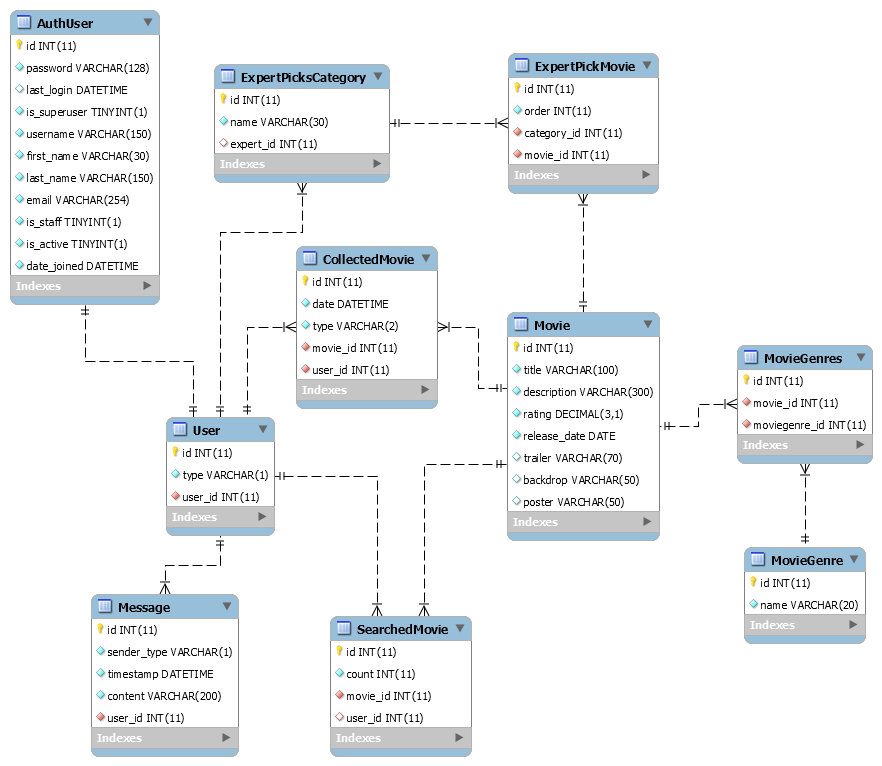
\includegraphics[width=\linewidth]{model.png}
\end{figure}

\subsection{Шема релационе базе података}

\textbf{User}(\underline{id}, type, user\_id)
\vspace{0.2cm}

\textbf{Message}(\underline{id}, sender\_type, timestamp, content, user\_id)
\vspace{0.2cm}

\textbf{MovieGenre}(\underline{id}, name)
\vspace{0.2cm}

\textbf{Movie}(\underline{id}, title, description, rating, release\_date, trailer, backdrop, poster)
\vspace{0.2cm}

\textbf{MovieGenres}(\underline{id}, movie\_id, moviegenre\_id)
\vspace{0.2cm}

\textbf{ExpertPicksCategory}(\underline{id}, name, expert\_id)
\vspace{0.2cm}

\textbf{ExpertPickMovie}(\underline{id}, order, category\_id, movie\_id)
\vspace{0.2cm}

\textbf{CollectedMovie}(\underline{id}, date, type, movie\_id, user\_id)
\vspace{0.2cm}

\textbf{SearchedMovie}(\underline{id}, count, movie\_id, user\_id)

\section{Табеле}
\subsection{User}

Садржи податке о кориснику сервиса. Ради искоришћења аутентификације имплементиране за радни оквир 
\textit{Django}, ова табела поред додатних поља садржи и референцу ка креираном кориснику у оквиру
табеле \textit{User} радног оквира која енкапсулира основне податке о кориснику, као и податке за
аутентификацију.

\vspace{0.5cm}

\noindent
\setcellgapes{4pt}
\makegapedcells
\begin{tabularx}{\linewidth}{|X|X|X|X|}
    \hline
    \textbf{Name} & \textbf{Datatype} & \textbf{Is PK} & \textbf{Is FK} \\
    \hline
    id & integer & Yes & No \\
    \hline
    user\_id & integer & No & Yes \\
    \hline
    type & varchar(1) & No & No \\
    \hline
\end{tabularx}

\subsection{Message}

Садржи информације о историји порука за одређеног корисника.

\vspace{0.5cm}

\noindent
\setcellgapes{4pt}
\makegapedcells
\begin{tabularx}{\linewidth}{|X|X|X|X|}
    \hline
    \textbf{Name} & \textbf{Datatype} & \textbf{Is PK} & \textbf{Is FK} \\
    \hline
    id & integer & Yes & No \\
    \hline
    user\_id & integer & No & Yes \\
    \hline
    type & varchar(1) & No & No \\
    \hline
    sender\_type & varchar(1) & No & No \\
    \hline
    timestamp & timestamptz & No & No \\
    \hline
    content & jsonb & No & No \\
    \hline
\end{tabularx}

\subsection{Movie}

Садржи податке о филмовима референцираним у оквиру апликације који се прикупљају из
екстерне базе филмова \textit{The Movie Database}. Примарни кључ има исту вредност као
и шифра филма у екстерној бази.

\vspace{0.5cm}

\noindent
\setcellgapes{4pt}
\makegapedcells
\begin{tabularx}{\linewidth}{|X|X|X|X|}
    \hline
    \textbf{Name} & \textbf{Datatype} & \textbf{Is PK} & \textbf{Is FK} \\
    \hline
    id & integer & Yes & No \\
    \hline
    title & varchar(100) & No & No \\
    \hline
    description & varchar(200) & No & No \\
    \hline
    rating & decimal(3, 1) & No & No \\
    \hline
    release\_date & date & No & No \\
    \hline
    trailer & varchar(70) & No & No \\
    \hline
\end{tabularx}

\subsection{ExpertPickMovie}

Садржи информације које филмове су експерти предложили и за коју категорију.

\vspace{0.5cm}

\noindent
\setcellgapes{4pt}
\makegapedcells
\begin{tabularx}{\linewidth}{|X|X|X|X|}
    \hline
    \textbf{Name} & \textbf{Datatype} & \textbf{Is PK} & \textbf{Is FK} \\
    \hline
    id & integer & Yes & No \\
    \hline
    order & integer & No & No \\
    \hline
    category\_id & integer & No & Yes \\
    \hline
    movie\_id & integer & No & Yes \\
    \hline
\end{tabularx}

\subsection{MovieGenre}

Садржи имена жанрова филмова који постоје у бази.

\vspace{0.5cm}

\noindent
\setcellgapes{4pt}
\makegapedcells
\begin{tabularx}{\linewidth}{|X|X|X|X|}
    \hline
    \textbf{Name} & \textbf{Datatype} & \textbf{Is PK} & \textbf{Is FK} \\
    \hline
    id & integer & Yes & No \\
    \hline
    name & varchar(20) & No & No \\
    \hline
\end{tabularx}

\subsection{ExpertPickCategory}

Садржи списак свих категорија и експерте који су задужени за одговарајућу категорију. 

\vspace{0.5cm}

\noindent
\setcellgapes{4pt}
\makegapedcells
\begin{tabularx}{\linewidth}{|X|X|X|X|}
    \hline
    \textbf{Name} & \textbf{Datatype} & \textbf{Is PK} & \textbf{Is FK} \\
    \hline
    id & integer & Yes & No \\
    \hline
    name & varchar(30) & No & No \\
    \hline
    expert\_id & integer & No & Yes \\
    \hline
\end{tabularx}

\subsection{SearchedMovie}

Садржи информације о филмовима које су корисници претраживали, као и број претраживања једног филма од стране корисника.

\vspace{0.5cm}

\noindent
\setcellgapes{4pt}
\makegapedcells
\begin{tabularx}{\linewidth}{|X|X|X|X|}
    \hline
    \textbf{Name} & \textbf{Datatype} & \textbf{Is PK} & \textbf{Is FK} \\
    \hline
    id & integer & Yes & No \\
    \hline
    count & integer & No & No \\
    \hline
    user\_id & integer & No & Yes \\
    \hline
    movie\_id & integer & No & Yes \\
    \hline
\end{tabularx}

\subsection{CollectedMovie}

Садржи информације о филмовима које су корисници одгледали или ставили у листу за гледање, као и датум када су то учинили.

\vspace{0.5cm}

\noindent
\setcellgapes{4pt}
\makegapedcells
\begin{tabularx}{\linewidth}{|X|X|X|X|}
    \hline
    \textbf{Name} & \textbf{Datatype} & \textbf{Is PK} & \textbf{Is FK} \\
    \hline
    id & integer & Yes & No \\
    \hline
    date & date & No & No \\
    \hline
    type & varchar(2) & No & No \\
    \hline
    user\_id & integer & No & Yes \\
    \hline
    movie\_id & integer & No & Yes \\
    \hline
\end{tabularx}

\subsection{MovieGenres}

Садржи за сваки филм којим жанровима припада.

\vspace{0.5cm}

\noindent
\setcellgapes{4pt}
\makegapedcells
\begin{tabularx}{\linewidth}{|X|X|X|X|}
    \hline
    \textbf{Name} & \textbf{Datatype} & \textbf{Is PK} & \textbf{Is FK} \\
    \hline
    id & integer & Yes & No \\
    \hline
    moviegenre\_id & integer & No & Yes \\
    \hline
    movie\_id & integer & No & Yes \\
    \hline
\end{tabularx}

\end{document}
